\section{Dimensionen, Schnitte und Kontouren}
\subsection{Dimensionen}

$$f: \mathbb{D}_f (\subseteqq  \rreal^{\cbl{\bm{m}}}) \longrightarrow \mathbb{W}_f (\subseteqq  \rreal^{\cgn{\bm{n}}})$$


\begin{ctabular}{O l}
    \cbl{\bm{m}}    & Anzahl Dimensionen von ${\mathbb{D}_f}$, wobei $\cbl{\bm{m}}$ ${\in \nnatural }$\\
    \cgn{\bm{n}}    & Anzahl Dimensionen von ${\mathbb{W}_f}$, wobei $\cgn{\bm{n}}$ ${\in \nnatural }$\\
    \vec{f}         & wenn Output vektoriell
\end{ctabular}

\warn{Variablen sind abhängig von einander!}


\subsubsection*{Multi-Variat:}

\begin{minipage}[t]{0.48\columnwidth}
    \textbf{${f}$} ist "Multi-Variat", wenn:
\begin{itemize}
    \item Input mehrdimensional ist
    \item Output mehrdimensional ist
    \item Input \textbf{und} Output\\
    mehrdimensional sind
\end{itemize}

\end{minipage}
\hfill
\begin{minipage}[t]{0.48\columnwidth}
    \textbf{${f}$} ist \crd{nicht} "Multi-Variat", wenn:
\begin{itemize}
    \item Input \textbf{und} Output Skalare sind
\end{itemize}
\end{minipage}

\subsubsection{Raumzeit}

$$\left.\begin{array}{r@{}}
    \text{Raum 3D ${(x;y;z)}$ }\rreal^3\\
    \text{Zeit 1D ${(t)}$ }\rreal^1
\end{array}\right\rbrace \rreal^{1}\times \rreal^3 = \text{Raumzeit 4D} \text{ } (t;x;y;z)$$

\subsubsection{Stationärer Fall}
$${t \rightarrow \infty \rightarrow \text{Stationär}}$$
$${\crd{T(x;y;z) \enspace\frac{\Delta{T}}{\Delta{t}} \rightarrow 0 }}$$


\subsubsection{Einheitsvektoren (Koordinatenvektoren)}

\begin{minipage}[c]{0.48\columnwidth}
    $$\hat{x}=\vec{i}=\cbl{\hat{i}}=\vec{{e}_1}=
\cbl{\begin{pmatrix}
    1 \\
    0 \\
    0
\end{pmatrix}}$$
$$\hat{y}=\vec{j}=\cgn{\hat{j}}=\vec{{e}_2}=
\cgn{\begin{pmatrix}
    0 \\
    1 \\
    0
\end{pmatrix}}$$
$$\hat{z}=\vec{k}=\crd{\hat{k}}=\vec{{e}_3}=
\crd{\begin{pmatrix}
    0 \\
    0 \\
    1
\end{pmatrix}}$$
\end{minipage}
\hfill
\begin{minipage}[c]{0.48\columnwidth}
    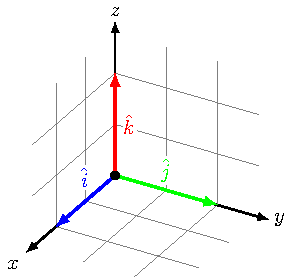
\includegraphics[width=\columnwidth]{images/einheitsvektoren.pdf}
\end{minipage}

\subsection{Schnitte}
Schnitt = Restriktion $\rightarrow$ Teilmenge vom Definitionsbereich ${\mathbb{D}_f}$


\subsubsection{Partielle Funktion}

\begin{itemize}
    \item Nur \textbf{eine} Variable ist frei! (wählbar)
    \item \textbf{Alle} anderen Variablen sind fix!
    \item[] \warn{$\mathbb{W}_f$ Analyse!}
\end{itemize}

\example{Schnitte}

\begin{minipage}[t]{0.48\columnwidth}
    \textbf{x-Linien}
    \begin{itemize}
        \item Fläche wird geschnitten mit Ebene, die parallel zur x,z-Ebene liegt
        \item Bestehen aus den $(x;y;z)$ Punkten\\
        $(x ; y_0 ; f(x;y_0))$
        \item ${x}$-Wert ist variabel
        \item ${y}$-Wert ist fixiert $\Leftrightarrow$ $y_0 = 2$
    \end{itemize}
    
    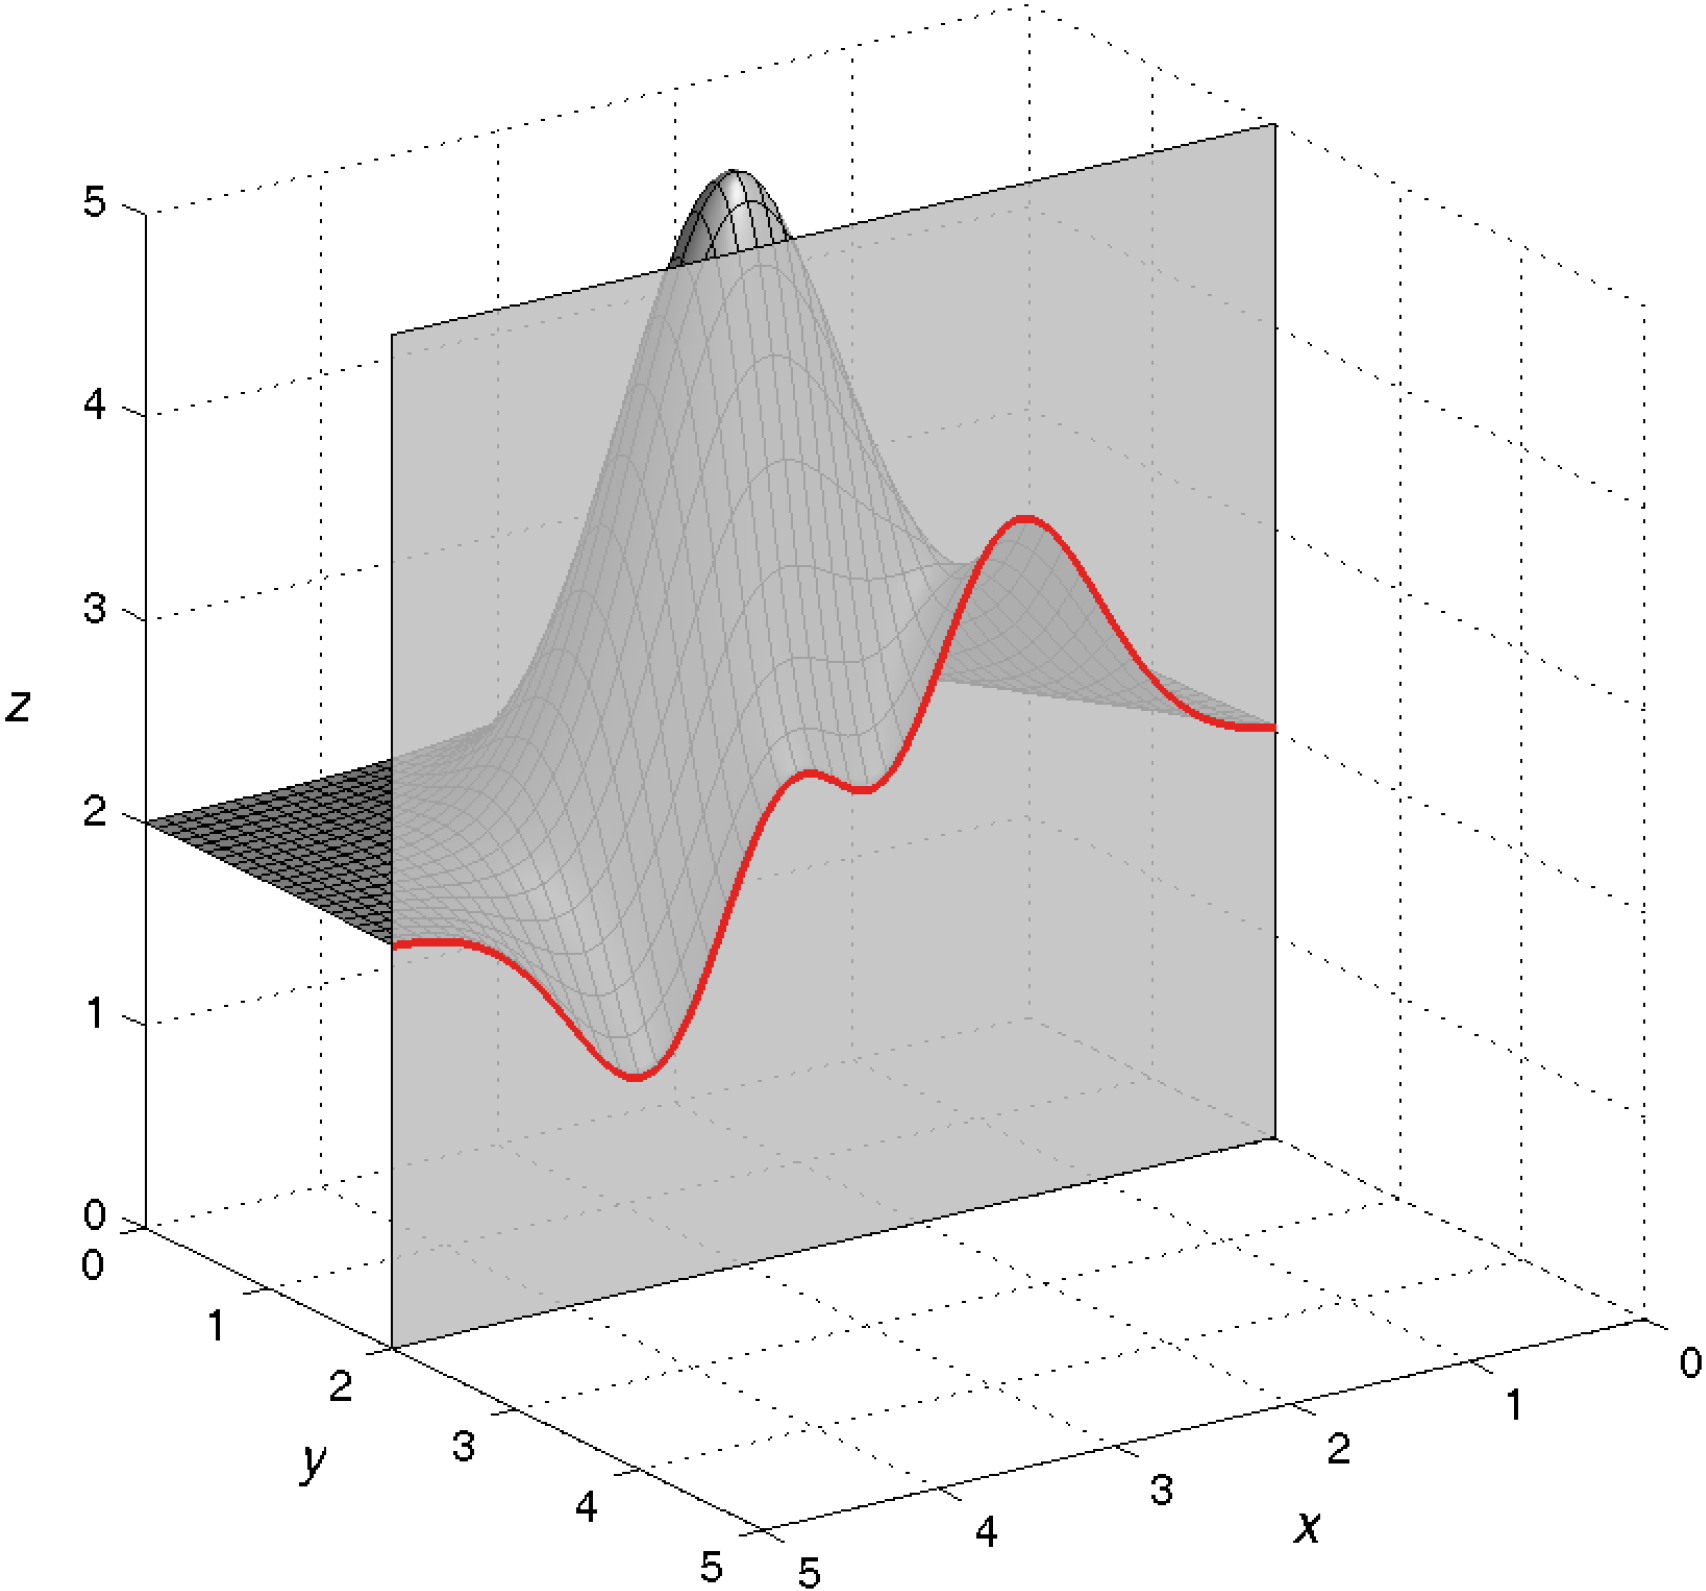
\includegraphics[width=\columnwidth]{images/schnitt_y0.png}
\end{minipage}
\hfill
\begin{minipage}[t]{0.48\columnwidth}
    \textbf{y-Linien}
    \begin{itemize}
        \item Fläche wird geschnitten mit Ebene, die parallel zur y,z-Ebene liegt.
        \item Bestehen aus den $(x;y;z)$ Punkten\\
        $(x_0;y;f(x_0;y))$
        \item $x$-Wert ist fixiert $\Leftrightarrow$ $x_0 = 3$
        \item $y$-Wert ist variabel
    \end{itemize}
    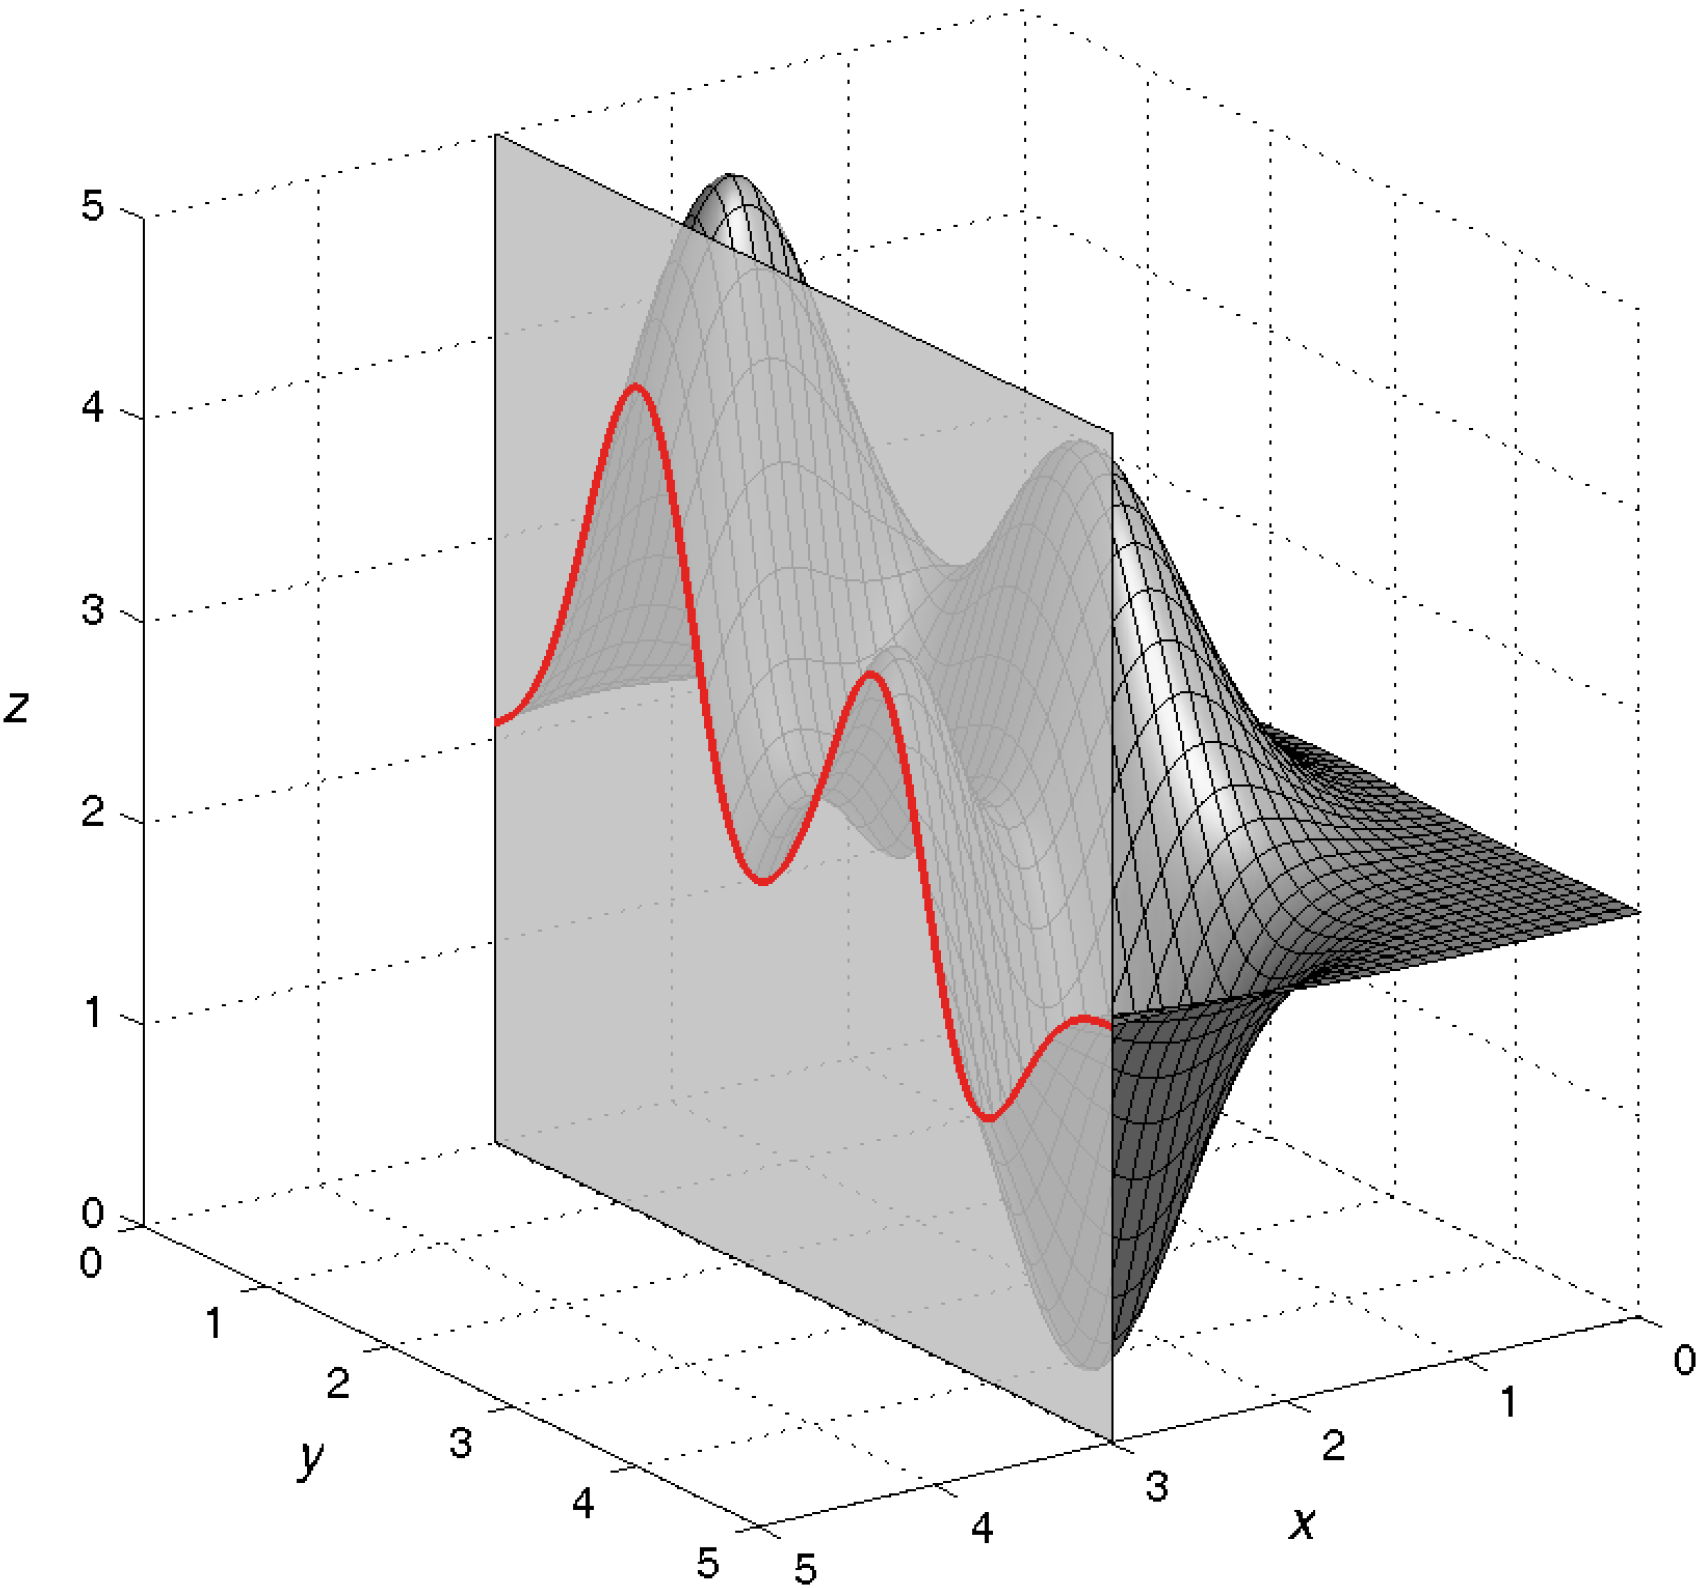
\includegraphics[width=\columnwidth]{images/schnitt_x0.png}
\end{minipage}

\subsubsection{Bedingungen}

\begin{tabular}{l l l}
    \textbf{Initial}bedingungen & $\rightarrow$ & Beziehen sich auf die \textbf{Zeit}\\
    \textbf{Rand}bedingungen & $\rightarrow$ & Beziehen sich auf \textbf{räumliche Ebenen}
\end{tabular}

\subsection{Kontouren, Levelsets, Niveaulinien, Höhenlinen, ...}
Bei \textbf{Kontouren}, \textbf{Levelsets}, \textbf{Niveaulinien} oder \textbf{Höhenlinien}
ist der \textbf{Output} der Funktion ${f}$ \textbf{konstant}.
$$\vec{y} = \vec{f}(\vec{x}) = \text{const. wobei } \vec{x} \subset \mathbb{D}_f$$

\example{Höhenlinien}

    \textbf{Kontouren (Höhenlinien)}
    \begin{itemize}
        \item Fläche wird geschnitten mit einer Ebene, die parallel zur x,y-Ebene liegt
        \item Bestehen aus den $(x;y;z)$ Punkten $(x ; y; f(x;y) = z_0)$
        \item $x$-Wert ist variabel
        \item $y$-Wert ist variabel
        \item ${z}$-Wert ist fixiert $\Leftrightarrow$ $z_0 = 3$
    \end{itemize} 

\begin{minipage}[t]{0.48\columnwidth}
    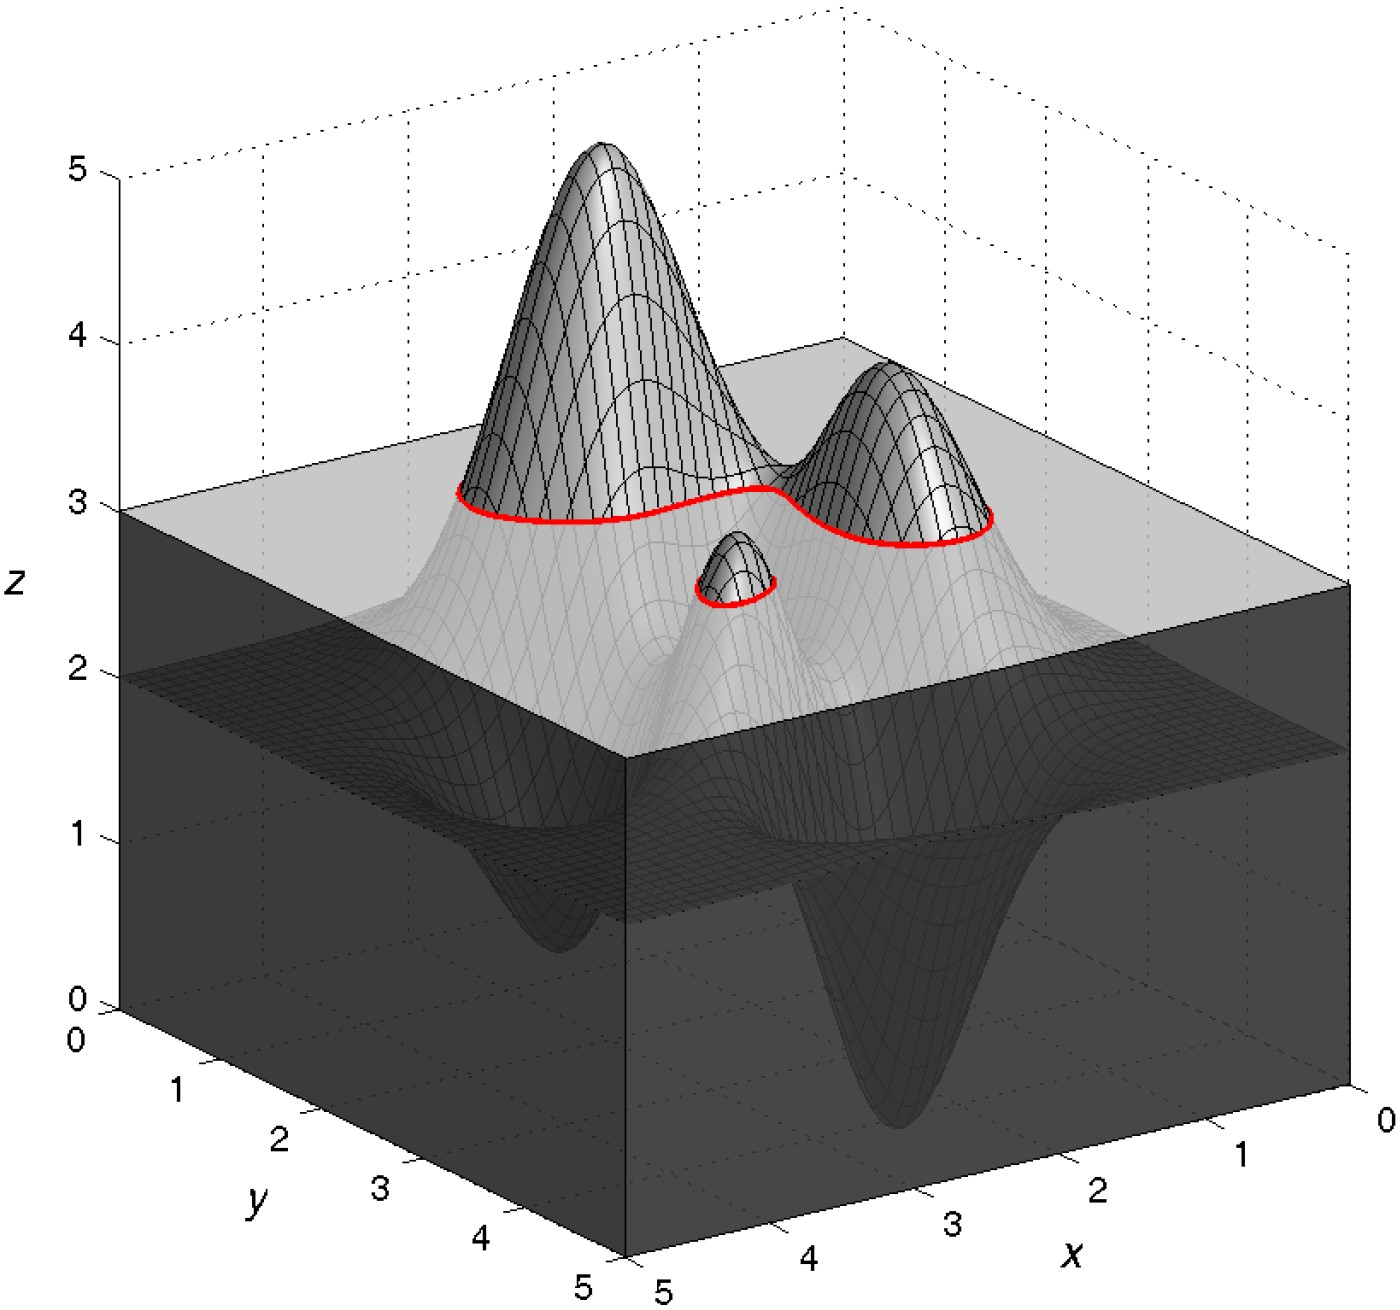
\includegraphics[width=\columnwidth]{images/niveaulinien1.png}
\end{minipage}
\hfill
\begin{minipage}[t]{0.48\columnwidth}
    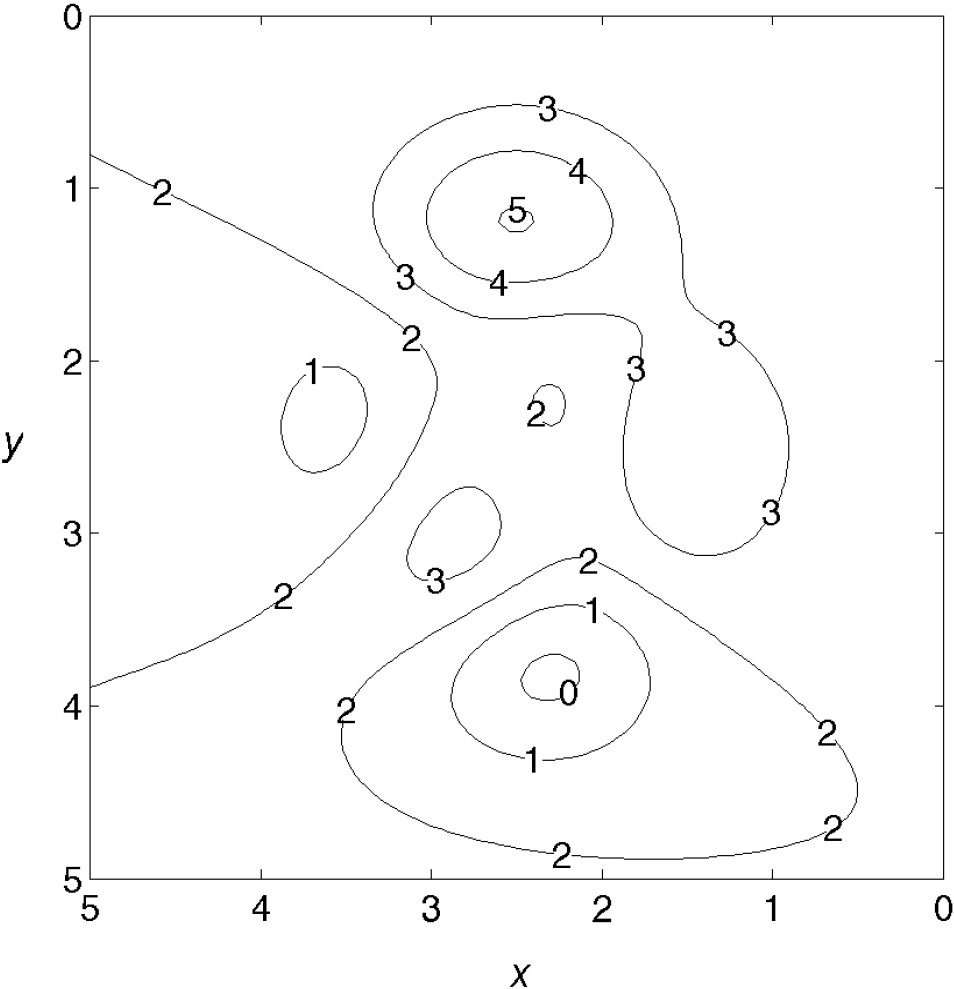
\includegraphics[width=\columnwidth]{images/niveaulinien2.png}
\end{minipage}